\chapter{基于话题演化的演员社交推广行为影响力模型}
\label{model}

\section{引言}
本章是对第四章应用的优化应用,使倾向值模型更合理的应用在演员推广行为的分析中。不但结合话题演化规律,将话题根据电视剧上映时间分成平稳期和爆发期,分别在两个时期分析演员的推广行为和推广策略,而且将更多会影响电视剧话题热度的因素考虑在内,使分析结果更具有可靠性。

\section{电视剧话题演化规律}
研究发现,微博热点话题在传播过程中,不仅关键词高度集中、受外界环境影响显著,而且传播具有周期性。话题周期一般包括话题发生、话题发展、话题高潮和话题消退四个阶段 \cite{赵龙文2013基于意见领袖参与行为的微博话题热度预测研究}。在话题发展的过程,起引导作用的是大量“意见领袖”的参与。意见领袖是指在人际传播网络中的“活跃分子”,他们经常为他人提供信息、施加影响,在大众传播效果的形成过程中起着重要的中介或过滤的作用,他们将信息扩散给受众,形成信息传递的两级传播 \cite{http://baike.baidu.com/link?url=VE98zoCZ8paIYRmIAvmZIwv9F_u8nXU-5yLru_SxRWG5i4-sl2h59-eJu6Op6w10-ZsQAyrQpv7mizJS3FOs2YtnNeqklulN0vvuSKM4vS-vGbZunTtAPQirQPfb0Cg7}。

统计发现,电视剧微博话题演化符合话题演化的基本特征,具有一定的周期特性,如图5-1,电视剧“柠檬初上”的话题发展正是经历了话题发生、话题发展、话题高潮和话题消退的过程。在电视剧话题演化的过程中,演员充当了意见领袖的作用,他们不仅拥有很庞大的粉丝群体,还有很大的社交影响力。他们发布的微博信息往往能受到高度关注,在电视剧话题发展过程中,演员发挥了核心作用。在电视剧话题发展过程中有三个重要时间节点导致了电视剧话题向下一阶段的发展,分别是电视剧上映时间确定、首集播出时间、首轮播出结束。在电视剧上映时间确定之前,演员会不时发些电视剧相关信息包括电视剧拍摄进度、拍摄期间趣事、角色定妆照等信息的微博,提前宣传使电视剧话题在微博产生。当电视剧上映时间确定后,主演通常都会发微博宣传电视剧,推动话题发展和酝酿,吸引粉丝和普通用户注意上映时间,吸引第一拨群众。当电视剧首轮播放第一集之后,演员发布微博来吸引观看用户参与电视剧剧情、角色相关的讨论,用户也因为看过电视剧,在微博上更愿意参与到话题讨论中去,带来话题热度的大发展。演员和用户的这种行为会持续到电视剧首轮播放结束后几天,之后话题因为其时效性,最终走向消退。

\begin{figure}[!htbp]
\centering
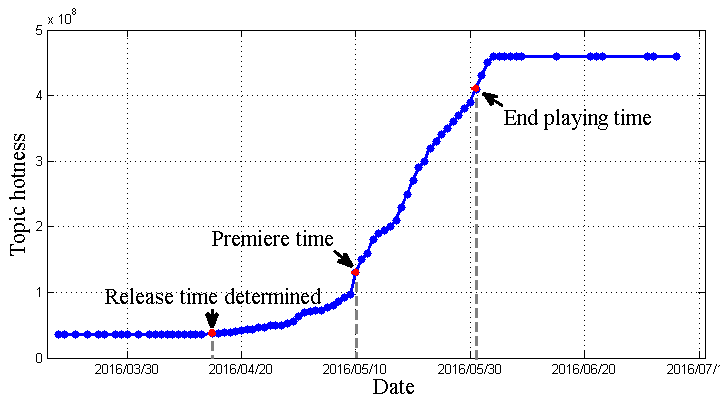
\includegraphics[height=3.6cm,width=8cm]{2}
\caption{Topic evolution of ``\textit{Ningmeng Chushang}''}
\end{figure}

电视剧话题出现和发展期相对于话题爆发和消退期存在本质上的差别,即电视剧是否已经上映,带来用户对电视剧的内容了解的差异和参与方式的不同,进而导致话题热度发展不同。因此,本文中将电视剧话题根据电视剧是否上映分成两个主要时期,上映前为平稳期,上映后为爆发期。在电视剧话题的整个发展过程中,因为电视剧所处宣传期不同,演员在微博上不同时期的推广方式也会有差异。例如,对发布推广微博的时间,如图3-1,在平稳期夜晚发布微博很少,白天不同时间发布微博数量比较平稳。但是在爆发期,在电视剧上映前后演员会有一个发布微博的高峰。在此时间发布微博不但能维持既有用户群观看电视剧、参与到电视剧话题讨论,还能吸引和号召新用户观看当天剧情。在不同时期演员发布推广微博的互动模式也有差异,从图3-2可以看出,与平稳期相比,爆发期演员会更多的与官方微博互动。因为当电视剧上映后,官方微博会发布更多的微博,包括剧情讨论、角色讨论、剧照、下集预告等等。因此,研究演员在不同时期推广策略的有效性是非常有必要的。

\section{倾向值匹配算法}
\subsection{混淆变量及推广策略}
在倾向值匹配算法中,应该控制混淆变量使得混淆变量在策略组和非策略组分布相似,这样才能更好的分析策略的效果。考虑到影响一条微博在微博中热度的因素有很多,除了演员的推广策略本身,还受演员本身属性及电视剧属性等的影响,因此,本章中我们选用如表5-1中包括演员和电视剧相关属性的信息作为混淆变量,使分析结果更具有可靠性。

\begin{table}[!htbp]
\centering
\caption{Baseline Covariates}=
\begin{tabular}{|c|c|} \hline
Type & Characteristics\\ \hline
\multirow{3}{*}{Actors} & number of fans\\% \hline
& gender\\% \hline
& number of works\\ \hline
\multirow{2}{*}{TV series} & cast\\% \hline
&score \\ \hline
\end{tabular}
\end{table}

因为话题演化的周期特性,以及在电视剧宣传的不同时期演员都需要在微博中进行推广,所以在平稳期和爆发期分别分析演员推广的有效策略更为合理。在算法应用中,将演员行为数据按照电视剧上映时间分成两部分,对两个时期的数据分别应用倾向值匹配算法,其中,推广策略如表5-2。同样地,我们定义每一项推广策略都是一项策略t,其值为T。在我们的研究中,$T={0,1}$,其中“1”代表采用这项策略,“0”代表不采用这项策略。同时定义与采用干预t的微博的影响力作为输入$Y(t)$,混淆变量为$X$,当研究一项推广策略时,另外的推广模式下的推广策略会作为混淆变量加入$X$。

\section{结果分析}
将倾向值匹配算法分别应用在演员推广的平稳期和爆发期,结果如下:
1)平稳期推广策略效果分析。推广策略有效性和t检验结果如表5-3所示。从表中可以看出,与在早晨和中午发布微博相比,在晚上发布微博的效果更好。用户晚上通常会花较多的时间在社交网络上,对他们而言,晚上发布的推广微博有更大的概率被他们看到。对互动模式而言,发布原创微博带来的推广效果要明显远远好于其他互动模式。与之相反,与官微互动和与其他人互动带来的推广效果较差。因为这种微博不能很好的表达演员自己的情感和想法,而且此时电视剧并未上映,粉丝参与电视剧推广微博更多的是因为演员,而不是因为剧情,因此对能更好表达演员自己想法和情感的原创微博会带来更好的粉丝参与度。与此同时,与其他主演互动的模式没有明显好的推广效果。

\begin{table*}[!htbp]
\centering
\caption{Effects of promotion strategies in steady period and outbreak period}
\begin{tabular}{|c|c|c|c|c|c|} \hline
\multicolumn{3}{|c}{Steady Period}& \multicolumn{3}{|c|}{Outbreak Period}\\ \hline
Strategy &\hfil ATT & \tabincell{c}{T-test\\significance} & Strategy &\hfil ATT & \tabincell{c}{T-test\\significance}\\ \hline
morning & -0.141 & 0.267& morning & 0.222 & 0.410\\% \hline
afternoon & 0.023 & 0.837 & afternoon & 0.211 & 0.008\\% \hline
evening & 0.359 & 0.024 & evening & -0.176 & 0.004\\ \hline
actors & -0.088 & 0.561 &  actors & -0.078 & 0.302\\
official accounts & -0.318 & 0.002 & official accounts & -0.001 & 0.989\\% \hline
original microblog& 2.633 & 0.000 & original microblog& 1.860 & 0.000\\
others & -0.743 & 0.000 & others & -0.616 & 0.000\\ \hline
\end{tabular}
\end{table*}

2)爆发期推广策略效果分析。根据图5-3可以看出,在爆发期,下午发布的推广微博会带来更好的推广效果。在爆发期,演员通常在晚上会集中发很多微博,导致平均每条微博的粉丝参与度相对不高。从互动模式来看,发原创微博仍然是最有效的推广策略,原创微博需要演员投入更多的精力编写,同时更好的表达了他的想法和对粉丝参与的期望。而与其他人互动仍然效果最差,与官方微博和其他主演互动的推广效果并不显著。因此可知,在爆发期,演员在下午发布原创微博能获得更好的宣传效果。

\section{模型显著性及平衡性检验}
平衡性检验用来评估倾向值匹配模型是否恰当的进行了应用,包括分布计算各个策略下,所有混淆变量标准差在策略组和非策略组的平均值是否有显著差异,作累计分布图和分位数-分位数图(qq图)来看混淆变量在策略组和非策略组是否分布一致。表5-4显示了两个时期,在各个时间策略下混淆变量的标准偏差。平稳期的标准偏差值在0.001到0.073之间,爆发期的标准偏差值在0.002到0.037之间,表明了策略组和非策略组的匹配样本的平均值分布一致。图5-6以是否采用原创微博策略下微博所属演员粉丝量、所属演员作品数、所属电视剧评分、所属电视剧阵容的累计分布图和分位数-分位数图来刻画在采用策略组和非策略组的混淆变量的分布情况,从图中可以看出,平稳期和爆发期的策略组和非策略组的这几个连续混淆变量的分布都非常类似。因此,倾向值匹配算法在我们的数据中得到了适当的应用,结果准确。


\begin{figure}[h]
  \centering%
  \subcaptionbox{steady period}
    {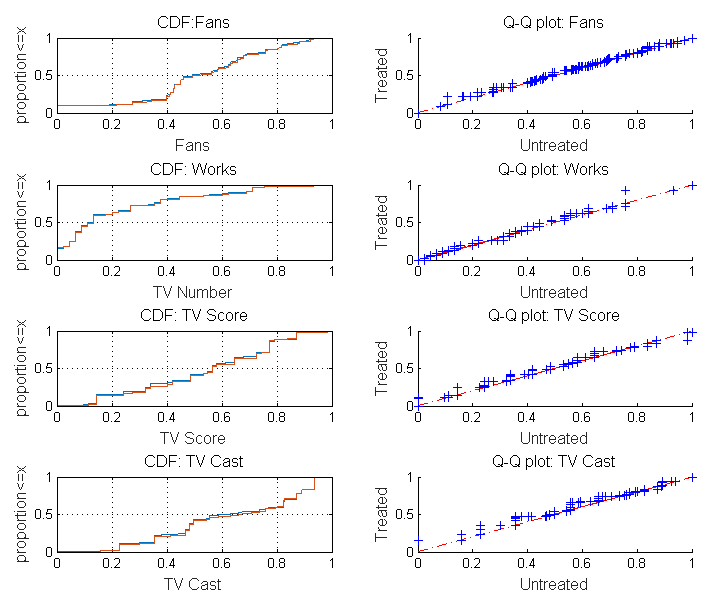
\includegraphics[height=9cm,width=8.7cm]{7}}
  \subcaptionbox{outbreak period}
    {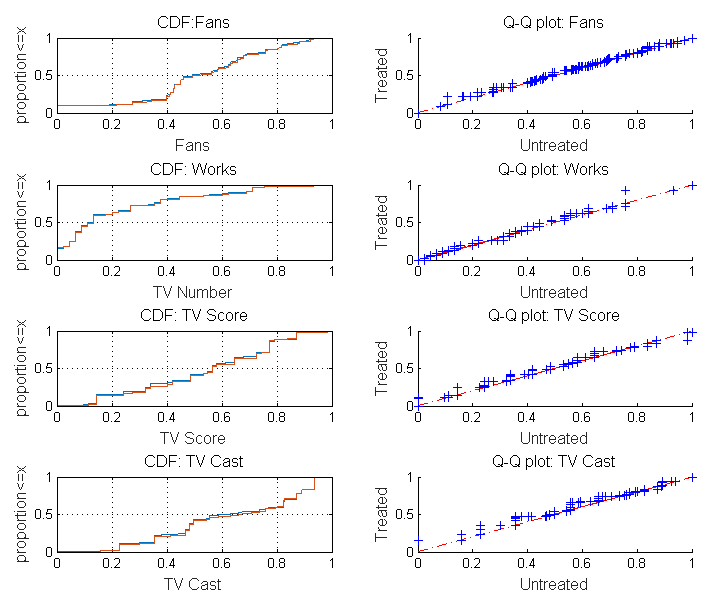
\includegraphics[height=9cm,width=8.7cm]{7}}
\caption{Comparing distribution of continuous covariate in propensity-score matched sample}
\end{figure}


\begin{table*}[!htbp]
\centering
\caption{Standardized difference of the mean of steady period and outbreak period}
\begin{tabular}{|c|c|c|p{0.1\textwidth}|c|c|c|p{0.1\textwidth}|} \hline
\multicolumn{4}{|c}{Steady Period}& \multicolumn{4}{|c|}{Outbreak Period}\\ \hline
&morning&afternoon&\hfil night & &morning&afternoon&\hfil night\\ \hline
actors&0.012&0.073&\hfil 0.058&actors&0.028&0.027&\hfil 0.008\\ \hline
\tabincell{c}{official\\accounts}&0.029&0.007&\hfil 0.001&\tabincell{c}{official\\accounts}&0.007&0.011&\hfil 0.003 \\ \hline
\tabincell{c}{original\\microblog}&0.053&0.006&\hfil 0.034&\tabincell{c}{original\\microblog}&0.008&0.003&\hfil 0.008\\ \hline
other&0.019&0.009&\hfil 0.047&other&0.018&0.006&\hfil 0.006\\ \hline
 \#works&0.006&0.023&\hfil 0.007&\#works&0.006&0.013&\hfil 0.007\\ \hline
gender&0.012&0.003&\hfil 0.054&gender&0.023&0.047&\hfil 0.010\\ \hline
\#fans&0.008&0.033&\hfil 0.003&\#fans&0.005&0.037&\hfil 0.002\\ \hline
cast&0.012&0.033&\hfil 0.032&cast&0.002&0.023&\hfil 0.003\\ \hline
score&0.030&0.049&\hfil 0.043&score&0.002&0.034&\hfil0.018\\ \hline
\end{tabular}
\end{table*}












